\subsection{Zusammenspiel mit Nagios}

Nagios dient zum Überwachen von Hosts und deren Services in komplexeren Infrastrukturen und bietet viele zusätzliche Features.
Es gibt einige essentielle Unterschiede zwischen den beiden Überwachungsanwendungen.
Während Munin mehr Wert auf die Visualisierung der Überwachungsdaten legt, kümmert sich Nagios intensiver um die Überwachungs- und Alarmierungslogik.
Beispielsweise überwacht Munin ständig die Überschreitung von den angegebenen Schwellwerten und schlägt ggf. Alarm.
Im Gegensatz hierzu wird bei Nagios mit Hard- und Soft-States gearbeitet, bei denen sich der Fehler erst durch mehrmaliges Überprüfen als "`True Positive"' beweisen muss.

Dies ist nur ein Beispiel für die überlegene Überwachungslogik von Nagios, doch Munin wurde nicht in der Absicht entwickelt mit Nagios zu konkurrieren.
Das genaue Gegenteil ist der Fall - Nagios und Munin können zusammenarbeiten.

Es ist durchaus denkbar, dass bereits ein Nagios-Überwachungssytem in der Netzwerkstruktur betrieben wird.
Eine zusätzliche Benachrichtigung von Fehlern bzw. Warnungen und die dezentrale Aufsplittung der Überwachung in zwei getrennte Systeme ist in den meisten Fällen ineffizient und daher nicht gewollt.

Deshalb gibt es die Möglichkeit die vorhandene Nagios-Instanz als "`Event-Handler"' für die von Munin festgestellten Überschreitungen von Schwellwerten zu verwenden.

Dabei wird, anstatt der Alarmierung durch Emails, ein passives Check-Ergebnis mittels \pictext{send\_nsca} an den Nagios Server versendet.
Dieser nimmt das Ergebnis entgegen und benachrichtigt die entsprechenden Benutzer.
Damit Nagios solche passiven Ergebnisse aufnehmen kann, muss sich auf dem Nagios-Server ein NSCA-Daemon (Nagios Service Check Acceptor) befinden, der auf dem entsprechenden Port auf die Benachrichtigungen wartet.

In folgender Abbildung wird ein beispielhafter Aufbau eines solchen Systems gezeigt, welches die Kommunikation zwischen Nagios und Munin verdeutlichen soll:

\begin{figure}[ht]
	\centering
	   \fbox{\includegraphics[width=0.9\textwidth]{bilder/nsca.png}}
		\caption{Zusammenarbeit von Munin und Nagios}
		\label{nsca}
\end{figure}

\begin{enumerate}
\item Der Munin-Master sammelt in periodischen Abläufen die Messwerte ab, welche ständig von den Munin-Nodes selbst ermittelt werden.
\item Die Messwerte werden vom Master überprüft.
\item Bei einer Überschreitung wird, anstatt einer Email, das Tool \pictext{send\_nsca} dazu verwendet, den Nagios-Server darüber zu benachrichtigen.
\item Der auf dem Nagios-Server laufende NSCA-Daemon nimmt das Ergebnis des Munin-Masters als passives Check-Ergebnis entgegen und filtert nochmals nach seinen eigenen Benachrichtigungs- und Eskalationsregeln.
\item Bei einer notwendigen Alarmierung nimmt Nagios Kontakt mit den zuständigen Benutzern auf.
\end{enumerate}

\subsection{Vergleich der Visualisierung mit Nagios}

Nagios bietet standardmäßig keine Visualisierung der Überwachungsdaten an.

Durch verschiedene Addons lässt sich dies jedoch nachträglich hinzufügen.

Solche Addons sind zum Beispiel:
\begin{itemize}
\item Nagiosgraph 

\begin{figure}[ht]
	\centering
	   \fbox{\includegraphics[width=0.9\textwidth]{bilder/nagiosgraph.png}}
		\caption{Visualisierung der Performancedaten mit Nagiosgraph}
		\label{nagiosgraph}
\end{figure}

\item drraw

\begin{figure}[ht]
	\centering
	   \fbox{\includegraphics[width=0.85\textwidth]{bilder/drraw.png}}
		\caption{Visualisierung der Performancedaten mit drraw}
		\label{drraw}
\end{figure}

\newpage
\item NagiosGrapher

\begin{figure}[ht]
	\centering
	   \fbox{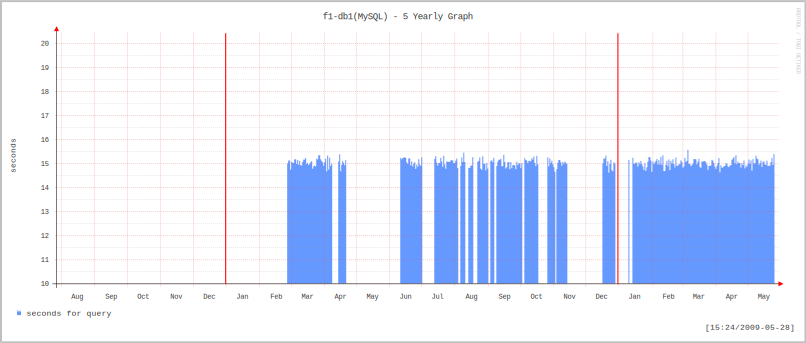
\includegraphics[width=0.9\textwidth]{bilder/nagios.png}}
		\caption{Visualisierung der Performancedaten mit NagiosGrapher}
		\label{nagios}
\end{figure}

\item Perf2rrd

\begin{figure}[ht]
	\centering
	   \fbox{\includegraphics[width=0.85\textwidth]{bilder/perf2rdd.png}}
		\caption{Visualisierung der Performancedaten mit Perf2rrd}
		\label{perf2rdd}
\end{figure}
\end{itemize}

Allgemein lässt sich sagen, dass die Visualisierung der Überwachungsdaten durch Nagios als unerfahrener Benutzer deutlich aufwändiger ist als mit Munin, da alleine die Entscheidung für ein Addon und dessen Konfiguration bis zum ersten Graphen länger als eine vollständige Munin Installation dauert.
Dafür stehen mit den Nagios-Visualisierungs-Addon mehr Möglichkeiten zur Verfügung, indem zum Beispiel die Performanzedaten länger als ein Jahr gespeichert werden können, wie in vorheriger Abbildung \ref{nagios}, mit einem Zeitverlauf über fünf Jahren, gezeigt.

